\section{Introduction}

\begin{figure}[b]
	\centering
	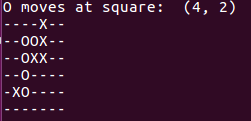
\includegraphics[ width = \columnwidth ]{Assets/argmax_9}
	\caption{ The board representations that the user sees on output }
	\label{fig:argmax_10}
\end{figure}

$M$-$N$-$K$ games are a popular method of entertainment, played by people of all ages.
They derive their name from being played on boards of size $M \times N$, and they are won by forming a sequence of length $K$.
Popular forms of these games are Tic-Tac-Toe and Connect 4, which would be a (3, 3, 3) and (6, 7, 4) $M$-$N$-$K$ game respectively.
Wei ji Ma~\cite{weiJiMa} discusses $M$-$N$-$K$ games and lists out the problems that have been ``solved\footnote{By ``solved'' we mean that it is known whether the first player to act will win or draw given optimal play from both sides.}'' in this domain.
He provides a table describing the regimes of $M$, $N$, and $K$ which are known to be solved, shown in Table~\ref{weiJiMa}.
This is where deep learning can really assist humanity in trying to show what conditions are viable for victory as the board size grows.

\begin{table}
\begin{tabular}{@{}l|l}
\emph{\textbf{$K$ values}} & Win on \emph{\textbf{$ M \times N$ board}} \\
\hline
1 & Always\\
\hline
2 &  iff $n > 2$\\
\hline
3 &  iff $m \geq 3$ and $n \geq 4$\\
\hline
4 & iff ($m \geq 5$ and $n \geq 6$) or ($m = 4$ and $n \geq 9$)\\
\hline
5 & if $m = n \geq 15$; not if $n \leq 6$ \\
\hline
6 & not if $m = n = 6$ (conjecture: never)\\
\hline
7 & (conjecture: never)\\
\hline
$\geq$ 8 & never \\
\end{tabular}
\caption{Wei Ji Ma's table describing solved states of MNK games.
Some results have been proven, and others are labelled conjectures}
\label{tab:weiJiMa}
\end{table}

From work such as AlphaGo Zero~\cite{alphaGoZero}, DeepMind has found a set of new opening moves that grandmasters in the domain of Go had not even considered viable opening moves.
However, the successes in this domain have shown that networks can see patterns and potential moves that even the strongest human players may not consider.
The problem with neural networks is that the solutions that they arrive at might not be understandable to humans, and this causes a problem when a human is asked to evaluate whether or not the network is making decisions \emph{for the right reasons}.

Approaching the $M$-$N$-$K$ games domain, we hope to work towards answering a few things that will help understanding the $M$-$N$-$K$ domain as well as help improve human-understanding of neural networks.
We wanted to:
\begin{enumerate}\itemsep0em
\item Investigate if a neural network can form winning strategies (particularly for larger boards which are not known to be solved).
\item Look at how different agents performed in this domain.
Our project created both search-based and CNN-based agents.
\item Use these agents to test human-understandability of explanations and network architectures.
\end{enumerate}
